\section{Diagrama de Classes}

O diagrama de classes é uma das peças de modelação que mais fazem sentido utilizar, porque é uma representação da estrutura e das relações das classes que servem de modelo para objetos.

Estes definem todas as classes que o sistema necessita de ter e é a base para a construção dos restantes diagramas de comunicação, sequência e de estados.
Com a utilização deste diagrama é possível visualizar a representação da estrutura do sistema recorrendo ao conceito de classes e relações. Este modelo resulta de um processo de seleção onde são identificados os objetos relevantes do sistema em estudo e que se pretende descrever no seu ambiente.

Optou-se pela utilização deste diagrama, pois deste modo consegue-se visualizar como cada classe se relaciona com as restantes, tendo como objetivo a satisfação dos requisitos funcionais definidos para o sistema em estudo. A legibilidade do mesmo permite que a transição para implementação de código seja facilmente interpretada.

\begin{figure}[H]
\centerline{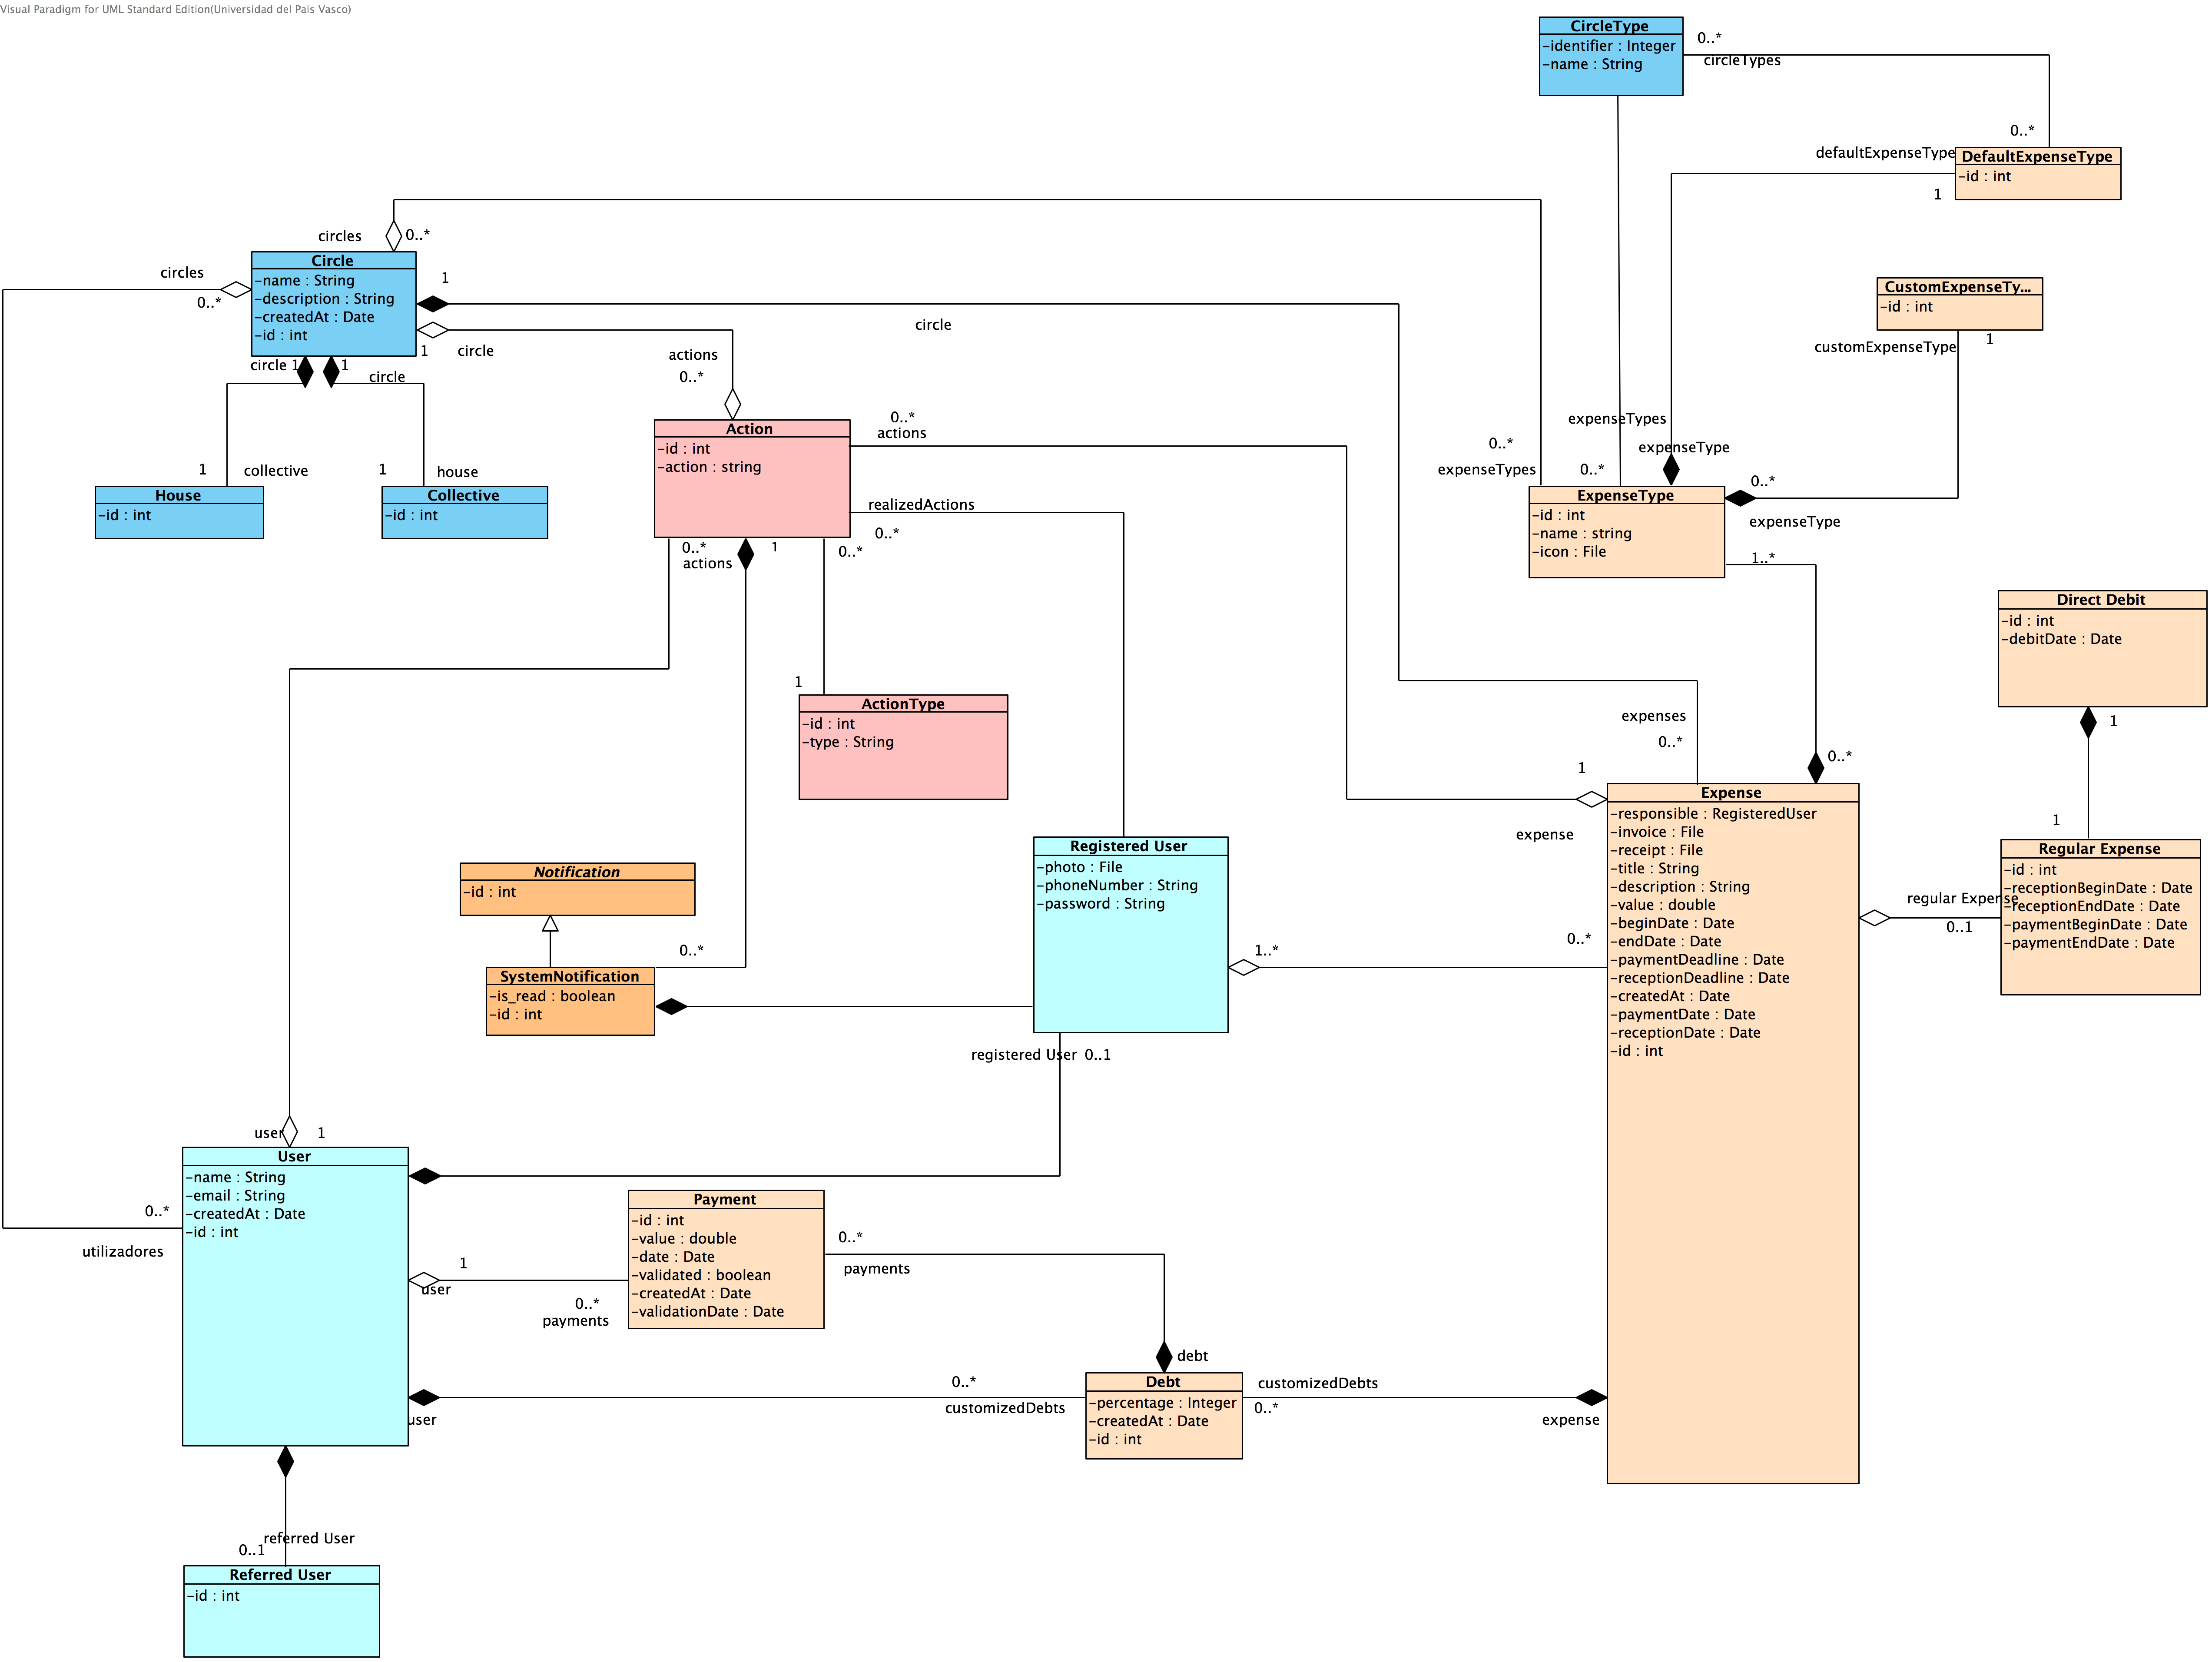
\includegraphics[width=1\textwidth]{images/modeling/diagramaClasses}}
\caption{Diagrama do modelo de domínio}
\label{fig:classDiagram}
\end{figure}

Inicialmente optou-se pela utilização de herança, contudo, quando se estava a fazer a modelação reparou-se que não estava a ser feita a correta reutilização dos recursos, sendo necessário instanciar o objeto para o poder reutilizar. Um exemplo simples é o caso do utilizador referenciado. Supondo que existe um utilizador que é referenciado com o email abc@abc.com. Se for implementada a herança, quando ele se regista é preciso instanciar um utilizador registado. Com composição, pode-se utilizar o \textit{design pattern state}, que faz com que não seja necessário uma nova instância, mudando apenas o estado de utilizador registado para utilizador referenciado.

Normalmente, deve-se preferir a composição sobre a herança, mas obviamente que existem exceções. Basicamente, usa-se a herança quando se sabe que a superclasse não vai variar, porque caso contrário será necessário alterar todas as classes que a implementam. Neste caso, está-se claramente a ver que a herança era a pior escolha em todos os casos, porque, quer-se um relacionamento do tipo "tem um", por exemplo, o utilizador registado tem um utilizador.

De seguida serão apresentadas todas as classes do sistema de uma forma mais detalhada, explicando os seus relacionamentos e a sua cardinalidade.
\begin{itemize}
	\item \textbf{\textit{User}}\\
	O \textit{registered user} e o \textit{referred user} têm um \textit{user}. Aqui tem-se a composição de ambos devido ao que foi explicado na introdução desta secção.
	Sendo o objetivo desta aplicação a partilha de despesas entre várias pessoas, então, a classe \textit{user} tem uma \textit{debt} que a relaciona com a classe \textit{expense}. Esta classe tem ainda outro relacionamento com a classe \textit{payment} que o relaciona com a classe \textit{debt}. Isto ocorre porque um utilizador pode fazer vários pagamentos para pagar uma despesa.

	\item \textbf{\textit{Circle}}\\
	A classe \textit{house} e \textit{collective} têm um \textit{circle}. Com isto, verifica-se que um \textit{circle} tem um ou mais \textit{users}, mas os \textit{users} podem não estar em nenhum \textit{circle}.
	O \textit{circle} tem um ou mais \textit{expenseTypes}, que serão utilizados para criar as despesas para um determinado círculo. Esta classe contém \textit{expenses} efetuadas por membros do círculo.

	\item \textbf{\textit{Expense}}\\
	Esta é a classe mais importante do sistema, uma vez que se relaciona com todas as classes. Este é bastante significativo porque indica os utilizadores que têm pagamentos em dívidas realizadas num determinado círculo.

	\item \textbf{\textit{Payment}}\\
	Os \textit{payments} indicam os utilizadores que têm pagamentos numa determinada dívida. Um \textit{user} pode ter vários \textit{payments}, porque pode realizar vários pagamentos para pagar uma dívida.

	\item \textbf{\textit{Debt}}\\
	Como já deu para perceber anteriormente, a classe \textit{Debt} indica a dívida que um utilizador tem numa determinada despesa. Um \textit{user} pode ter várias \textit{debts}, mas cada \textit{debt} pertence a um \textit{user}. Do mesmo modo, uma \textit{expense} pode ter zero ou várias \textit{debts}, mas cada \textit{debt} é relativa apenas a uma \textit{expense}.

	\item \textbf{\textit{Action}}\\
	A classe \textit{action} é gerada sempre que qualquer utilizador realizar uma determinada tarefa no sistema.

	\item \textbf{\textit{Notification}}\\
	As notificações serão geradas a partir das \textit{actions} realizadas pelos \textit{users}.

	\item \textbf{\textit{Regular Expense}}\\
	Esta classe é criada sempre que um utilizador quiser criar uma despesa regular, que basicamente o alerta sobre as próximas faturas, para que este não se esqueça de criar as despesas. Com isto, é possível criar uma despesa sem esforço para o utilizador, porque os atributos da despesa são preenchidos com os atributos da despesa regular.

	\item \textbf{\textit{Expense Type}}\\
	Esta classe tem os tipos de despesa que são apresentados no momento em que se criam despesas, porque é obrigatório que cada despesa tenha um tipo de despesa para se efetuar uma organização de despesas mais eficaz na lógica de negócio.

	\item \textbf{\textit{Circle Type}}\\
	Esta classe armazena os tipos de despesa que são apresentados no círculo no momento da sua criação. As que aparecem ao utilizador são as \textit{default expense types}, mas caso queira criar uma nova será adicionada ao \textit{custom expense type}.

\end{itemize}
